\documentclass[10pt]{scrreprt}
\usepackage{hyperref}
\usepackage{graphicx}
\graphicspath{ {./figures/} }
\usepackage[utf8]{inputenc}
\usepackage[T1]{fontenc}
\usepackage[]{ragged2e}
\usepackage[]{blindtext}
\usepackage{amsmath}
\usepackage[doublespacing]{setspace}
\usepackage[a4paper, left=2cm, right=2cm, top=2cm, bottom=3cm]{geometry}
\usepackage{amsmath}
\usepackage{mathtools}

\begin{document}
\chapter{EventFilter Query Language}
The following gives a short introduction into a newly proposed query langue to create OPC UA EventFilter.
The OPC Foundation specifies OPC UA EventFilter in the OPC UA Specification Part 4:Services. EventFilter consists of
a selectClauses that defines a list of values to be returned from a filtered event and a whereClause that defines a
ContentFilter that contains criteria which have to be met to receive a notification about the event. The values listed in the
selectCaluses are defined as SimpleAttributeOperands, so that the selectClauses consists of one or multiple
SimpleAttributeOperands. The ContentFilter is a collection of operators where each of them features a corresponding set of operands.

\section{Structure of the Query Language}
In accordance to the EventFilter definition, the query language is split into a SELECT and a WHERE statement.
Since the whereClause can describe a complex structure of operators, the corresponding statement can be rather complex and confusing.
To increase the usability of the language,
it introduces the FOR statement as an additional element that only occurs within the language. Consequently,
the concept of OPC UA EventFilter is not altered. The novelty of the FOR statement are references for operators and
operands. As a result, the WHERE statement can be simplified by referencing further operands or operators as elements,
which are then resolved within the FOR statement.

References can be used to link elements, either declared in the FOR statement or in the WHERE statement, to one
concrete element listed in the FOR statement. While multiple elements can reference one particular element, each reference
can only be resolved once. Since ElementOperands point to one ContentFilterElement inside the ContentFilterElementArray,
they can be seen as a reference from one operator to another. However, the logic of EventFilters
allows such references only for the OR and the AND operator. References that are used to describe ElementOperands can be freely chosen,
since they are replaced by the ContentFilterElementArrayIndex when constructing the EventFilter.


The example below should illustrate the logic of such references. Lines 1-4 specify
the selectClauses of the filter. Each additional operand of the selectClauses is separated by a comma. The ContentFilter
is defined from line 5 on. Its basic structure features an OR operator (line 6), which references a
GREATHERTHAN operator with \$”ref\_1”. The corresponding operator is then resolved in line 8 and
includes a reference to an operand (\$”ref\_2”). The concrete operand is then
declared in line 9 by dereferencing \$”ref\_2”:=. As last element, the OR operator has an OFTYPE operator which
references a NodeId defined with reference \$42.

\begin{addmargin}[60pt]{0pt}
    $
   1: \text{   } SELECT \newline
   2: \text{   } \text{PATH “/Message”,} \newline
   3: \text{   } \text{PATH “/0:Severity”,} \newline
   4: \text{   } \text{PATH “/EventType”} \newline
   5: \text{   } WHERE \newline
   6: \text{   } \text{OR(\$"ref\_1", \text{OFTYPE } \$42)} \newline
   7: \text{   } FOR \newline
   8: \text{   } \text{\$"ref\_1"}\coloneqq \text{PATH "/Severity"}  \text{ GREATERTHAN } \text{\$"ref\_2"} \newline
   9: \text{   } \text{\$"ref\_2"}\coloneqq \text{UINT32 } 10 \newline
   10: \text{   } \$42\coloneqq ns=1;i=5003
    $
\end{addmargin}

Since both, references and ElementOperands specify a reference to either an operand or an operator, they have an equal notation.
Both are defined by setting a \$ in front of either a number or, a string surrounded by quotation marks.
However, they have to be resolved by extending the initial reference with $\coloneqq$, followed by either an operand or operator
 (see e.g. \$”ref\_1” declared in line 6 is then resolved in line 8). It is
important to consider that references to operands are only allowed for Operators and references to Operators are only
allowed by ElementOperands to create valid EventFilters. Additionally, references can be nested, so that an
initially referenced operators can contain further references to operands (The OR operator in line 6 references the
GREATERTHAN operator in line 8, which in turn references the LiteralOperand in line 9).

\section{BNF of the Query Language for EventFilter}
The BNF used for these examples uses `<´ and `>´ to mark symbols, `[´ and `]´ to identify optional paths and `|´ to identify alternatives.
If the ‘(‘ and ‘)’ symbols are used, it indicates sets. Lastly, the '\{' and '\}' symbols indicate that an element occurs zero or multiple times. Expressions surroundet by '\'' have to be matched exactly.



In addition not all elements are resolved down to the smallest element. Such elements are String-, JsonString-, Number, ByteString, Guid and relativePath expressions. The Query Language allows any element to be part of a string except
single quotation marks. Quotation marks have to be escaped with ///\("\). JsonStrings correspond to the OPC UA Json encoding. Since the query language implementation uses the open62541 Json parser, limitations and escape characters from this parser have to be
considered within the query language. Currently, the usage of JsonStrings for LiteralOperands is limited to OPC UA Variants. Other elements with restrictions related to open62541 parsers are relative-path-elements,
Guids, ByteStrings and NodeIds so that the corresponding escape characters and limitations have to be considered. Lastly, Numbers can be any number, including negative values and numbers with decimal places.

\begin{tabbing}
<EventFilter> $\Coloneqq$ <SelectClauses> <ContentFilter>
\end{tabbing}
\begin{tabbing}
<SelectClauses> $\Coloneqq$ 'SELECT' \{<SimpleAttributeOperand> ','\} <SimpleAttributeOperand>
\end{tabbing}
\begin{tabbing}
<ContentFilter> $\Coloneqq$ <WhereClause> [<ForClause>]
\end{tabbing}
\begin{tabbing}
<WhereClause> $\Coloneqq$ 'WHERE' (<Operator> | <ElementReference>)
\end{tabbing}
\begin{tabbing}
<ElementReference> $\Coloneqq$ '\$' (\('"\)String\("'\) | 'Number')
\end{tabbing}
\begin{tabbing}
<Operator> $\Coloneqq$ \\ \hspace{11mm} <SingleOperandOperator> \\ \hspace{10mm} | <TwoOperandsOperator> \\ \hspace{10mm} | <BetweenOperator> \\ \hspace{10mm} | <InListOperator>  \\ \hspace{10mm} | <BranchOperator>
\end{tabbing}
\begin{tabbing}
<SingleOperandOperator> $\Coloneqq$ ('OFTYPE' | ('ISNULL' | '0=') | ('NOT' | '!')) <Operand>
\end{tabbing}
\begin{tabbing}
<TwoOperandsOperator> $\Coloneqq$ \\ \hspace{10mm} <Operand> \\ \hspace{10mm} ( \\ \hspace{12mm} ('GREATERTHAN' | 'GT' | '>') \\ \hspace{10mm}
| ('EQUALS' | 'EQ' | \('"\)==\("'\)) \\ \hspace{10mm} | ('LESSTHAN' | 'LT' | '<')
\\ \hspace{10mm} | ('GREATEROREQUAL' | 'GE' | \('"\)>=\("'\)) \\ \hspace{10mm} | ('LESSOREQUAL' | 'LE' | \('"\)<=\("'\)) \\ \hspace{10mm} |
('LIKE' | \('"\)<=>\("'\)) \\ \hspace{10mm} | ('CAST' | '->')
\\ \hspace{10mm} | ('BITAND' | '\&') \\ \hspace{10mm} | ('BITOR' | 'v') \\ \hspace{10mm} ) \\ \hspace{10mm} <Operand>
\end{tabbing}
\begin{tabbing}
<BetweenOperator> $\Coloneqq$ <Operand> 'BETWEEN' '['<Operand>, <Operand>']'
\end{tabbing}
\begin{tabbing}
<InListOperator> $\Coloneqq$ <Operand> 'INLIST' '[' \{<Operand> ','\} <Operand>']'
\end{tabbing}
\begin{tabbing}
<BranchOperator> $\Coloneqq$ ('AND' | 'OR') '('<Operand> ',' <Operand>')'
\end{tabbing}
\begin{tabbing}
<Operand> $\Coloneqq$ \\ \hspace{12mm} <ElementOperand> \\ \hspace{10mm} | <SimpleAttributeOperand> \\ \hspace{10mm} | <LiteralOperand> \\ \hspace{10mm} | <ElementReference>
\end{tabbing}
\begin{tabbing}
<ElementOperand> $\Coloneqq$  <ElementReference>
\end{tabbing}
\begin{tabbing}
<SimpleAttributeOperand> $\Coloneqq$ \\ \hspace{10mm} ['TYPEID' <NodeId>] \\ \hspace{10mm} 'PATH' \('"\)relative path\("'\)\\ \hspace{10mm} ['ATTRIBUTE' 'Number'] \\ \hspace{10mm} ['INDEX' 'IndexRange']
\end{tabbing}
\begin{tabbing}
<LiterlOperand> $\Coloneqq$ 'JsonString' | <Literal>
\end{tabbing}
\begin{tabbing}
<Literal> $\Coloneqq$ \\ \hspace{10mm} (  (['STRING'] \('"\)String\("'\) ) \\
\hspace{10mm}| ('BOOL' ('True' | 'False' | 'false' | 'true' | '1' | '0') | ('True' | 'False' | 'false' | 'true')) \\ \hspace{10mm}|
['INT64'] "Number" \\ \hspace{10mm}| ('INT16' | 'UINT16' | 'UINT32' | 'INT32' | UINT64 ) 'Number' \\\hspace{10mm}| ['DOUBLE'] 'floating point' \\\hspace{10mm}| FLOAT 'floating point' \\\hspace{10mm}| ['NODEID'] <NodeId> \\\hspace{10mm}| 'SBYTE' {'-', 'Number'} \\\hspace{10mm}| 'BYTE' 'Number'
\\\hspace{10mm}| 'TIME' 'TimeValueString' \\\hspace{10mm}| 'GUID' 'GUID-String' \\\hspace{10mm}| 'BSTRING' \('"\)String\("'\) \\\hspace{10mm}| 'STATUSCODE' (\('"\)String\("'\)| 'Number') \\\hspace{10mm}| 'EXPNODEID' '"ExpandedNodeIdString"' \\\hspace{10mm}| ['QNAME'] '"relative-path-element"' \\\hspace{10mm}| 'LOCALIZED' '"String"')
\end{tabbing}
\begin{tabbing}
<ForClause> $\Coloneqq$ 'FOR' <ReferencedElement> \{<ReferencedElement>\}
\end{tabbing}
\begin{tabbing}
<ReferencedElement> $\Coloneqq$ ElementReference '$:=$' (<Operand> | <Operator>)
\end{tabbing}
\begin{tabbing}
<NodeId> $\Coloneqq$ \\ \hspace{10mm} ['ns=' 'Number' ';']
\\ \hspace{10mm} ( 's=' '"String"'
\\ \hspace{10mm} | 'i=' 'Number'
\\ \hspace{10mm} | 'b=' '"ByteString"'
\\ \hspace{10mm} | 'g=' 'Guid')
\end{tabbing}



\section{Simple EventFilter Query Examples}
The following examples illustrate how to build the EventFilter from the open62541 EventFilter examples
(\url{https://github.com/open62541/open62541/blob/master/examples/events/client_eventfilter.c})
with the proposed query language.

\subsection{SelectClauses}
\label{SelectClauses}

Since all considered EvenFilter have identical SelectClauses, the corresponding
statetement is only explained once. Each selectClauses consists of a list of one or multiple SimpleAttributeOperands
which are separated by a comma:
\begin{equation}
    \label{eq:1}
    \begin{split}
        \text{SELECT } \\\
        \text{PATH "/Message",} \\\
        \text{PATH "/0:Severity",} \\\
        \text{PATH "/EventType"}
    \end{split}
\end{equation}


These representations illustrate the minimal required information to define a SimpleAttributeOperand, since the IndexRange of SimpleAttributeOperands is optional,
the QueryLanguage defines the BaseEventType as default value for the TypeDefinitionId and the attribute value is set as default value for the AttributeId.
In consequence, these two statements create identical SimpleAttributeOperands:

\begin{addmargin}[125pt]{0pt}
    $
    1: \text{   } \text{PATH "/Message"} \newline
    2: \text{   } \text{TYPEID i=2041 PATH "/Message" ATTRIBUTE 13} \newline
    $
\end{addmargin}

The following table clearifies the SimpleAttributeOperands defined in Equation \ref{eq:1}

\begin{table}[h]
    \centering
    \caption{SelectClauses}
    \label{tab:selectClauses}
    \resizebox{\columnwidth}{!}{%
        \begin{tabular}{|c|c|c|c|c|}
            \hline
            \textbf{TypeDefinitionNode} & \textbf{IncludesSubtypes} & \textbf{RelativePath} & \textbf{Attribute} & \textbf{IndexRange} \\ \hline \hline
            i=2041 (BaseEventType) & True & /Message   & 13 (Value) & N/A \\ \hline
            i=2041 (BaseEventType) & True & /0:Severity  & 13 (Value) & N/A \\ \hline
            i=2041 (BaseEventType) & True & /EventType & 13 (Value) & N/A \\ \hline
        \end{tabular}%
    }
\end{table}

\subsection{Complex Operators}
Since all Operators used for the tutorial \ref{ref:open62541 EventFilter Tutorial} only contain a maximum of two operands,
the following shortly illustrates the usage of the the InList and the Between operators which allow more than two operands:

\begin{addmargin}[60pt]{0pt}
    $
    WHERE \newline
    \text{OR(\$"ref\_1", \$"ref\_3")} \newline
    FOR \newline
    \text{\$"ref\_1"}:= \text{PATH "/Severity"}  \text{ BETWEEN } \text{ [ \$"ref\_2",  \text{UINT32 } 18]} \newline
    \text{\$"ref\_2"}:= \text{UINT32 } 10 \newline
    \text{\$"ref\_3"}:= \text{PATH "/Severity" }  \text{ INLIST } \text{ [ \$"ref\_2", \text{UINT32 } 120, \text{UINT32 } 140 ]}
    $
\end{addmargin}
The ContentFilter statement limits the Severity to be either between 10 and 18 (\$"ref\_1") or its value has
to be equal to 10, 120 or 140 (\$"ref\_3"). Table \ref{tab:InList and Between Operators} should clarify the exact structure of this ContentFilter,
where Element represents the index of an operator within the ContentFilterElementArray, Operator the OperatorType, Operand illustrates each operand within
the operator's operand array and Reference shows either the internally generated reference, or the reference set by the user. Since the query language allows to set references for operands, some elements listed in the
table do not have Element and Operator values. Depending on the number of operands for a concrete operator, Operand cells can also be empty.
The InList operator has an undetermined number of operands, so that the number of operands listed in such a table depends on the size of the declared list in the operator's statement.


\begin{table}[h]
    \centering
    \caption{\textbf{InList and Between Operators}}
    \label{tab:InList and Between Operators}
    \resizebox{\columnwidth}{!}{%
        \begin{tabular}{|c|c|c|c|c|c|c|}
            \hline
            \textbf{Element} & \textbf{Operator} & \textbf{Operand{[}0{]}} & \textbf{Operand{[}1{]}} & \textbf{Operand{[}2{]}} & \textbf{Operand{[}3{]}} & \textbf{Reference} \\ \hline \hline
            0 & OR     & ElementOperand = 1           & ElementOperand = 2 & & & operator\_reference\_0 \\ \hline
            1 & BETWEEN & \shortstack{ \\ SimpleAttributeOperand = \\ \text{'}NodeId: i=2041,\\ BrowsePath: “/Severity”,
                \\ Attribute: Value, \\ IndexRange: N/A\text{'}} & Reference = \text{'}ref\_2\text{'}       & LiteralOperand = \text{'}$18$\text{'} &            & ref\_1                 \\ \hline
            &  & LiteralOperand = \text{'}$10$\text{'}      &  & &                   & ref\_2                 \\ \hline
            2 & INLIST & \shortstack{ \\ SimpleAttributeOperand = \\ \text{'}NodeId: i=2041,\\ BrowsePath: “/Severity”,
                \\ Attribute: Value, \\ IndexRange: N/A\text{'}}      & Reference = \text{'}ref\_2\text{'}  & LiteralOperand = \text{'}$120$\text{'} &  LiteralOperand = \text{'}$140$\text{'}                  & ref\_3                 \\ \hline
        \end{tabular}%
    }
\end{table}

\subsection{open62541 EventFilter Tutorial}
\label{ref:open62541 EventFilter Tutorial}

The open62541 EventFilter tutorial gives an extensive introduction into the OPC UA EventFilter and how to implement them manually with the open62541 SDK. Since plenty of coding effort is required to create them,
the open62541 query languge enables an easy alternative with reduced effort. Each of the following cases illustrates a possible query to create an EventFilter for the corresponding case from
the tutorial. However, the usage of default values for SimpleAttributeOperands, multiple possibilities to declare operators and the referencing of operands and operators facilitates different queries to create identical EventFilter.


Each Case is structured as followed. First, the query statement is represented, afterwards, a figure depicts the structure of this EventFilter and lastly, the ContentFilterElementArray is clarified in a table which lists each operator and operand of the ContentFilter.
Since all cases have an equal SelectClauses, the SELECT statement has been illustrated in section \ref{SelectClauses}.


\subsubsection*{Case 0}
The query shown below creates an EventFilter that collects the values of the Serverity, the Message and the EventType, when the EventType's NodeId corresponds to either $i=5000$ or $ns=1;i=5001$.
\begin{addmargin}[125pt]{0pt}
    $
    SELECT \newline
    \text{PATH "/Message", PATH "/0:Severity", PATH "/EventType"} \newline
    WHERE \newline
    \text{OR(\$"ref\_1", \$"ref\_2")} \newline
    FOR \newline
    \text{\$"ref\_2"}:= \text{OFTYPE } ns=1;i=5003 \newline
    \text{\$"ref\_1"}:= \text{OFTYPE } i=3035 \newline
    $
\end{addmargin}

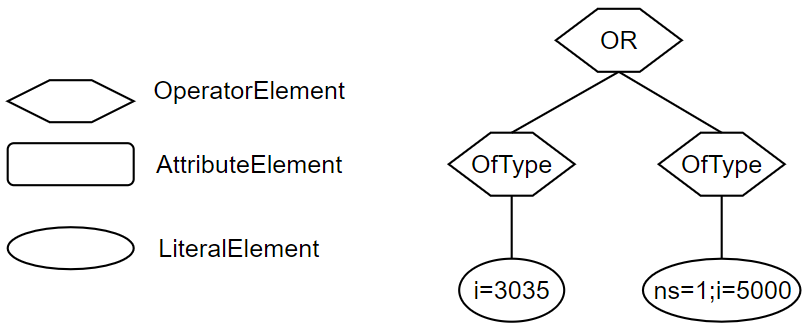
\includegraphics[width=\textwidth]{case_0.png}

\begin{table}[h]
    \centering
    \caption{\textbf{Case 0}}
    \label{tab:my-table}
    \resizebox{\columnwidth}{!}{%
        \begin{tabular}{|c|c|c|c|c|}
            \hline
            \textbf{Element} & \textbf{Operator} & \textbf{Operand{[}0{]}} & \textbf{Operand{[}1{]}} & \textbf{Reference} \\ \hline \hline
            0 & OR     & ElementOperand = 1           & ElementOperand = 2 & operator\_reference\_0 \\ \hline
            1 & OFTYPE & LiteralOperand = \text{'}$i=3035$\text{'} &                    & ref\_1                 \\ \hline
            2 & OFTYPE & LiteralOperand = \text{'}$ns=1;i=5000$\text{'}      &                    & ref\_2                 \\ \hline
        \end{tabular}%
    }
\end{table}

\subsubsection*{Case 1}
The query shown below creates an EventFilter that collects the values of the Serverity, the Message and the EventType, when the EventType's NodeId corresponds to $ns=1;i=5001$.


\begin{addmargin}[125pt]{0pt}
    $
    SELECT \newline
    \text{PATH "/Message", PATH "/0:Severity", PATH "/EventType"} \newline
    WHERE \newline
    \text{OFTYPE } ns=1;i=5001
    $
\end{addmargin}


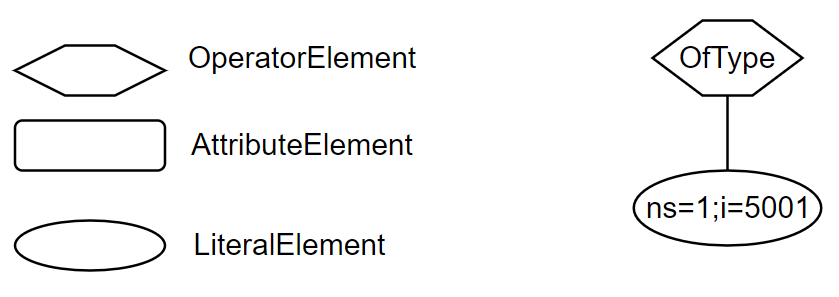
\includegraphics[width=\textwidth]{case_1.png}
\begin{table}[h]
    \centering
    \caption{\textbf{Case 1}}
    \label{tab:Case_1}
    \resizebox{\columnwidth}{!}{%
        \begin{tabular}{|c|c|c|c|c|}
            \hline
            \textbf{Element} & \textbf{Operator} & \textbf{Operand{[}0{]}} & \textbf{Operand{[}1{]}} & \textbf{Reference} \\ \hline \hline
            0 & OFTYPE & LiteralOperand = \text{'}$ns=1;i=5001$\text{'}      &                    & operand\_reference\_0                 \\ \hline

        \end{tabular}%
    }
\end{table}

\subsubsection*{Case 2}

The query shown below creates an EventFilter that collects the values of the Serverity, the Message and the EventType, when the EventType's NodeId corresponds to either $ns=1;i=5000$, $ns=1;i=5001$, $ns=1;i=5002$, $ns=1;i=5003$, $ns=1;i=5004$, $i=3035$.


\begin{addmargin}[125pt]{0pt}
    $
    SELECT \newline
    \text{PATH "/Message", PATH "/0:Severity", PATH "/EventType"} \newline
    WHERE \newline
    \text{OR}(\$\text{"first branch"}, \$\text{"second branch"}) \newline
    FOR \newline
    \$\text{"first branch"}:= \text{OR}(\$\text{"third branch"}, \$\text{"fourth branch"}) \newline
    \$\text{"second branch"}:= \text{OR}(\$1, \$2) \newline
    \$\text{"third branch"}:= \text{OR}(\$3, \$4) \newline
    \$\text{"fourth branch"}:= \text{OR}(\$5, \$6) \newline
    \$1:= \text{OFTYPE } ns=1;i=5000 \newline
    \$2:= \text{OFTYPE } \$7 \newline
    \$3:= \text{OFTYPE } ns=1;i=5002 \newline
    \$4:= \text{OFTYPE } ns=1;i=5003 \newline
    \$5:= \text{OFTYPE } \$8 \newline
    \$6:= \text{OFTYPE } \$9 \newline
    \$7:= \text{PATH "/0:SampleDeviceFailureEventType" ATTRIBUTE 1} \newline
    \$8:= ns=1;i=5004 \newline
    \$9:= \text{NODEID } i=3035 \newline
    $
\end{addmargin}

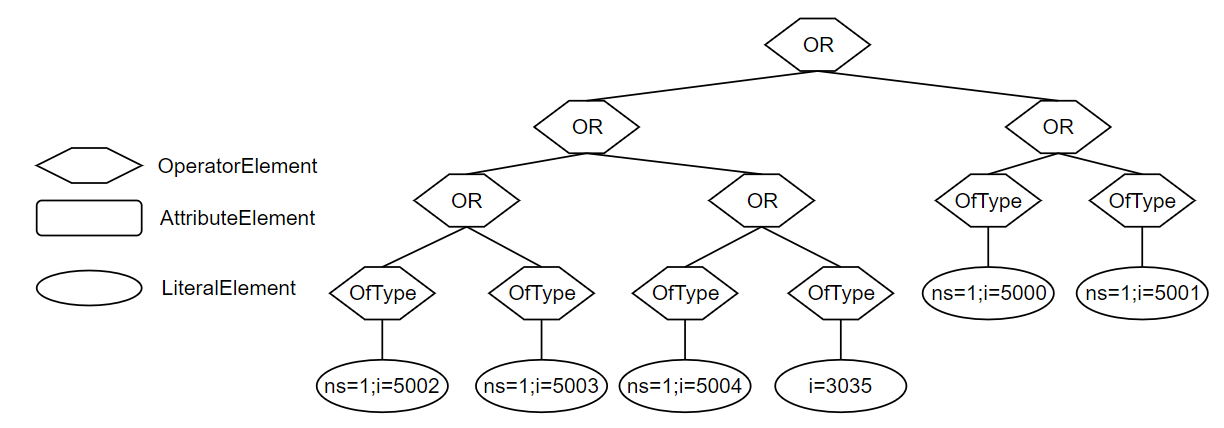
\includegraphics[width=\textwidth]{case_2.png}

\begin{table}[h]
    \centering
    \caption{\textbf{Case 2}}
    \label{tab:Case_2}
    \resizebox{\columnwidth}{!}{%
        \begin{tabular}{|c|c|c|c|c|}
            \hline
            \textbf{Element} & \textbf{Operator} & \textbf{Operand{[}0{]}} & \textbf{Operand{[}1{]}} & \textbf{Reference} \\ \hline \hline
            0 & OR & ElementOperand = \text{'}$1$\text{'}      & ElementOperand = \text{'}$2$\text{'}                   & operator\_reference\_0                 \\ \hline
            1 & OR & ElementOperand = \text{'}$3$\text{'}      & ElementOperand = \text{'}$4$\text{'}                   & first branch                 \\ \hline
            2 & OR & ElementOperand = \text{'}$5$\text{'}      & ElementOperand = \text{'}$6$\text{'}                   & second branch                 \\ \hline
            3 & OR & ElementOperand = \text{'}$7$\text{'}      & ElementOperand = \text{'}$8$\text{'}                   & third branch                 \\ \hline
            4 & OR & ElementOperand = \text{'}$9$\text{'}      & ElementOperand = \text{'}$10$\text{'}                   & fourth branch                \\ \hline
            5 & OFTYPE & LiteralOperand = \text{'}$ns=1;i=5000$\text{'}      &                    & 1                 \\ \hline
            6 & OFTYPE & Reference = \text{'}$7$\text{'}                     &                    & 2                 \\ \hline
            7 & OFTYPE & LiteralOperand = \text{'}$ns=1;i=5002$\text{'}      &                    & 3                 \\ \hline
            8 & OFTYPE & LiteralOperand = \text{'}$ns=1;i=5003$\text{'}      &                    & 4                 \\ \hline
            9 & OFTYPE & Reference = \text{'}$8$\text{'}      &                    & 5                 \\ \hline
            10 & OFTYPE & Reference = \text{'}$9$\text{'}      &                    & 6                 \\ \hline
            &       & \shortstack{ \\ SimpleAttributeOperand = \\ \text{'}NodeId: i=2041,\\ BrowsePath: “/0:SampleDeviceFailureEventType”,
                \\ Attribute: NodeId, \\ IndexRange: N/A\text{'}}       &                    & 7                 \\ \hline
            &  & LiteralOperand = \text{'}$ns=1;i=5004$\text{'}      &                    & 8                 \\ \hline
            &  & LiteralOperand = \text{'}$i=3035$\text{'}      &                    & 9                 \\ \hline
        \end{tabular}%
    }
\end{table}

\subsubsection*{Case 3}
The query shown below creates an EventFilter that collects the values of the Serverity, the Message and the EventType, when the EventType's NodeId corresponds to $ns=1;i=5001$, the literal value $99$ is equal to the literal value $99$ and
the event's severity value is greather than $99$.


\begin{addmargin}[125pt]{0pt}
    $
    SELECT \newline
    \text{PATH "/Message", PATH "/0:Severity", PATH "/EventType"} \newline
    WHERE \newline
    \text{AND}(\text{OFTYPE ns=1;i=5001}, \$3) \newline
    FOR \newline
    \$1:= 99 \text{ "==" }99 \newline
    \$2:= \text{ TYPEID i=5000 PATH "/Severity" GT } 99 \newline
    \$3:= \text{ AND }(\$1, \$2) \newline
    $
\end{addmargin}

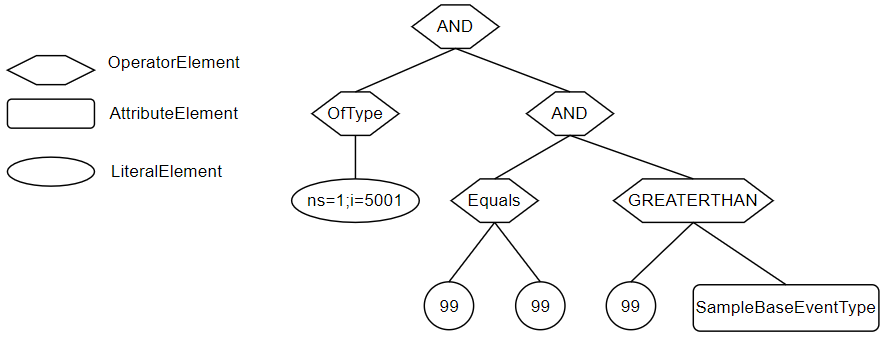
\includegraphics[width=\textwidth]{case_3.png}
\begin{table}[h]
    \centering
    \caption{\textbf{Case 3}}
    \label{tab:Case_3}
    \resizebox{\columnwidth}{!}{%
        \begin{tabular}{|c|c|c|c|c|}
            \hline
            \textbf{Element} & \textbf{Operator} & \textbf{Operand{[}0{]}} & \textbf{Operand{[}1{]}} & \textbf{Reference} \\ \hline \hline
            0 & AND & ElementOperand = \text{'}$1$\text{'}      &   ElementOperand = \text{'}$2$\text{'}                 & operator\_reference\_0                 \\ \hline
            1 & OFTYPE & LiteralOperand = \text{'}$ns=1;i=5001$\text{'}      &                    & operand\_reference\_0                 \\ \hline
            2 & AND & ElementOperand = \text{'}$3$\text{'}      &   ElementOperand = \text{'}$4$\text{'}                 & 3                 \\ \hline
            3 & EQUALS & LiteralOperand = \text{'}$99$\text{'}      &      LiteralOperand = \text{'}$99$\text{'}               & 1                \\ \hline
            4 & GREATERTHAN & LiteralOperand = \text{'}$99$\text{'}      &      \shortstack{ \\ SimpleAttributeOperand = \\ \text{'}NodeId: i=5000,\\ BrowsePath: “/Severity”,
                \\ Attribute: Value, \\ IndexRange: N/A\text{'}}               & 2                \\ \hline

        \end{tabular}%
    }
\end{table}


\subsubsection*{Case 4}

The query shown below creates an EventFilter that collects the values of the Serverity, the Message and the EventType, when the EventType's NodeId corresponds to $ns=1;i=5000$ and
the event's severity value is greather than $99$.


\begin{addmargin}[35pt]{0pt}
    $
    SELECT \newline
    \text{PATH "/Message", PATH "/0:Severity", PATH "/EventType"} \newline
    WHERE \newline
    \text{AND}(\text{(OFTYPE ns=1;i=5000)}, \text{ TYPEID i=5000 PATH "/Severity" GREATERTHAN }99)
    $
\end{addmargin}

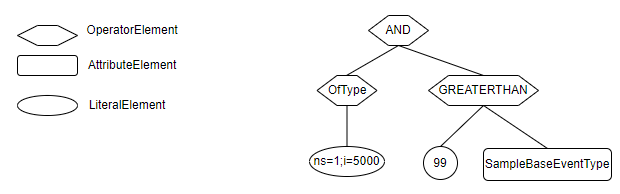
\includegraphics[width=\textwidth]{case_4.png}
\begin{table}[h]
    \centering
    \caption{\textbf{Case 4}}
    \label{tab:Case_4}
    \resizebox{\columnwidth}{!}{%
        \begin{tabular}{|c|c|c|c|c|}
            \hline
            \textbf{Element} & \textbf{Operator} & \textbf{Operand{[}0{]}} & \textbf{Operand{[}1{]}} & \textbf{Reference} \\ \hline \hline
            0 & AND & ElementOperand = \text{'}$1$\text{'}      &   ElementOperand = \text{'}$2$\text{'}                 & operator\_reference\_0                 \\ \hline
            1 & OFTYPE & LiteralOperand = \text{'}$ns=1;i=5000$\text{'}      &                    & operand\_reference\_0                 \\ \hline
            2 & GREATERTHAN & LiteralOperand = \text{'}$99$\text{'}      &      \shortstack{ \\ SimpleAttributeOperand = \\ \text{'}NodeId: i=5001,\\ BrowsePath: “/Severity”,
                \\ Attribute: Value, \\ IndexRange: N/A\text{'}}               & operand\_reference\_1                \\ \hline

        \end{tabular}%
    }
\end{table}

\end{document}